% This is samplepaper.tex, a sample chapter demonstrating the
% LLNCS macro package for Springer Computer Science proceedings;
% Version 2.20 of 2017/10/04
%
\documentclass[runningheads]{llncs}
%
\usepackage{graphicx}
\usepackage{scrextend}
\usepackage{listings}
\usepackage{float}
\usepackage{subfig}
\lstloadlanguages{C,C++,csh,Java}
% Used for displaying a sample figure. If possible, figure files should
% be included in EPS format.
%
% If you use the hyperref package, please uncomment the following line
% to display URLs in blue roman font according to Springer's eBook style:
% \renewcommand\UrlFont{\color{blue}\rmfamily}

\begin{document}
%
\title{Virtual reality and artificial intelligence as assistance in architectural planning}
%
\titlerunning{Artificial Intelligence and Virtual Reality in Architecture.}
% If the paper title is too long for the running head, you can set
% an abbreviated paper title here
%
\author{First Author\inst{1}\orcidID{0000-1111-2222-3333} \and
Second Author\inst{2,3}\orcidID{1111-2222-3333-4444} \and
Third Author\inst{3}\orcidID{2222--3333-4444-5555}}
%
\authorrunning{F. Author et al.}
% First names are abbreviated in the running head.
% If there are more than two authors, 'et al.' is used.
%
\institute{Princeton University, Princeton NJ 08544, USA \and
Springer Heidelberg, Tiergartenstr. 17, 69121 Heidelberg, Germany
\email{lncs@springer.com}\\
\url{http://www.springer.com/gp/computer-science/lncs} \and
ABC Institute, Rupert-Karls-University Heidelberg, Heidelberg, Germany\\
\email{\{abc,lncs\}@uni-heidelberg.de}}
%
\maketitle              % typeset the header of the contribution
%
\begin{abstract}
This paper proposes a system, which uses virtual reality (VR) and artificial intelligence (AI) technologies to support the process of designing architectural spaces -- both buildings and interiors -- by enabling an immersive design process that takes into account architectural laws, design patterns, common design choices, as well as previous interactions with a designer. The presented system gives users the possibility to design, configure and visualize their own space within a virtual reality environment. With the help of additional knowledge about the construction and infrastructure requirements and common design approaches, this system may significantly shorten and improve the design process. In addition, virtual reality helps users to get better understanding of the created space, while interact with the space is supported by AI techniques.

\keywords{Virtual Reality  \and Artificial Intelligence \and Architecture}
\end{abstract}
%
%
%
\section{Introduction}
The increasing use of interactive three-dimensional technologies, such as augmented reality (AR) and virtual reality (VR), for creating immersive multimodal human-computer interfaces has become possible mainly due to the significant progress in the efficiency of computing and graphics hardware, especially mobile devices. These techniques are gaining popularity, also thanks to the continually increasing bandwidth and availability of mobile computer networks, and increasingly sophisticated forms of presentation and interaction with 3D content available on end-user's equipment.

The constantly growing market of computer games is largely driven by the development of graphic hardware and applications based on three-dimensional user interfaces. However, the use of these techniques is not only limited to applications in the entertainment industry. They can be – and in fact are – successfully used in other areas, such as rapid prototyping of products, and simultaneous trainings. Standards such as COLLADA [ ], MPEG-4 [ ], U3D [ ] and VRML / X3D [ ] have been elaborated on the basis of standardization studies aimed at developing universal data formats for describing interactive three-dimensional VR / AR content available on the internet. These standards make it possible to use three-dimensional techniques on a completely new level, by encoding, transmitting over the network and presenting on the end-user's devices high-quality 3D interactive multimedia content. Users can use virtual environments available over the network in a similar way as their local equivalents.

The use of VR / AR techniques may not only lead to the implementation of improved versions of existing services, such as travel guides, e-learning systems, e-commerce applications or social and entertainment services. Remote access to 3D interactive content and multimedia services makes it possible to implement a class of new AR and VR services.

Digital services have been widely used in the architectural industry for a long time. Due to the necessity to improve the process of creating three-dimensional models, the quality and the manner of their subsequent presentation, as well as better parameterization of individual components (BIM) [ ], the number of applications of interactive three-dimensional content increases in the design process. However, it should be remembered that creating, searching and combining dispersed three-dimensional interactive content is much more complex and complicated than with standard software for creating 3D models. Currently used relationships between components within the digital content are limited to the basic meaning and form of the presentation. For better development of tools that can be used during the design process, spatial, temporal, structural or behavioral relationships should be introduced. This is possible through the use of semantic techniques. Even for content with relatively small structural complexity, such as HTML pages, the use of semantic techniques provides a significant increase in the ability to automatically process and integrate content.

This article presents a new approach to the use of digital services in the design process called SVDE. In this approach, a number of techniques have been used that improve the design of architectural spaces. Thanks to the additional use of semantic techniques, it allows appropriate organization and consistency of content that is shared and used by users. The presented approach is only aimed at simplifying and developing currently used design practices. The outline of the application architecture along with the prototype of the architectural space design tool, which was implemented as an extension to the Unity IDE [], was also presented.

The rest of the article is organized in the following way. Chapter 2 presents an overview of the state of the art in architectural design. In Chapter 3, the concept, requirements and general architecture of a distributed semantic design environment are discussed. Section 4 describes the implementation of the environment, presents a step-by-step design example and discusses possible further development directions.
Finally, section 5 concludes the paper.

\section{State of the Art}
The advancement of technology has allowed the development various approaches to the design of architectural spaces – both 2D and 3D. All these methods aim at reducing the amount of information necessary to provide at the design stage, as well as at decreasing the duration and complexity of the creation process. This is however often associated with the increase of the complexity of the software used in the design stage. Achieving the final effects is possible in several different ways presented below.
\subsection{2D Drawings}
2D design applications can be used to draw elements necessary to understand the designed space. These applications allow one to design spaces by using various 2D elements. Starting with simple lines in Autodesk AutoCAD applications and ending with complex multi-layer elements such as walls, e.g., in Graphisoft ArchiCAD or Autodesk Revit. The complexity of creating a space in this way depends on the degree of integration between the elements. For example, a room designed in AutoCAD requires more work on possible changes than Revit due to the lack of the ability to connect objects from different categories, such as toilet with a wall . Consequently, to move several lines that together form a wall in the first of these applications, the user must move all elements separately. On the other hand, the second application allows a user to move the wall with already associated facilities. There is the possibility of building a three-dimensional space in them, but the process is so complicated that they are used most often in conjunction with applications designed for 3D modeling. This solution gives some degree of freedom and introduces a hierarchy of architectural space design. Thanks to focusing on individual stages, it is possible to have a greater impact on the entire process, however this is also associated with the increase in the duration of the development of a space due to the need for amendments on both the 2D drawing and the 3D model.

\subsection{Visual Content Modeling}
The constant progress in technical capabilities combined with the needs of the computer games market have caused a significant increase in the availability of 3D modeling environments. There are many examples, but the most commonly used in both the entertainment and architectural industries are: 3dsMax, 3D-Coat, Blender, Maya, Modo, Rhino and Zbrush. The sophisticated environments intended for professional users are designed to allow any object to be created using a variety of techniques. However, it should be noted that their comprehensive capabilities are connected with the necessity of having experience in 3D modeling. Nonetheless, it is not always difficult to create 3D content. Proper orientation on specific applications and the limitation of the number of tools allows creating environments that are user-friendly in nature. Examples of this type of applications are: AutoCAD Civil 3D, Ghost Productions, SketchUp, and Sweet Home 3D. From the beginning, designed with specific industries in mind, they enable efficient creation of 3D content without the need for comprehensive knowledge in the field of modeling. However, it also involves a drastic reduction in the generality of the content creation process.

\subsection{Parametric Modeling Creation}
Very popular in the field of architecture, the parametric design trend, i.e., creating content only with the help of parameters, and not direct modeling using complicated tools that are included in 3D content creation applications. In this way, the creation process is limited to generating content on demand. With the help of ready-made templates, the person creating a given content needs only to ascribe certain parameters to specific elements, which does not require comprehensive knowledge. This limits the possibilities of creating flexible content to a large extent, but reduces the amount of information needed. These types of templates are most often made from a natural world such as the Voronoy diagram, which resembles arrangement of cells on a leaf. One of the applications that enables generation of this type of content is the Grasshopper extension to the Rhino software [].

\subsection{Augmented reality}
Augmented reality is a promising technique in the field of architectural design. However, currently the use of AR is this domain is low. This is due to several factors. Firstly, the available AR applications do not permit professional design of architectural spaces. Secondly, high cost and low availability of AR devices such as Magic Leap and Microsoft HoloLens, which facilitate interaction within the augmented reality environments discourage potential users and result in low market penetration. Devices which are widely available and popular, such as tablets and smartphones, do not provide quality and efficiency that would allow for effective creation of 3D architectural designs. Some companies provide their own design applications through application markets, such as the Google Play or the AppStore for mobile devices users, but they are mainly limited to browsing specific products in the existing space, without the possibility of using them at the design stage.

\subsection{Virtual reality}
Currently, there are no applications designed purely for the design of architectural spaces in virtual reality . Extensions are developed for modeling programs that enable to generate from an existing architectural model a VR environment in which the user can freely navigate. These tools, however, do not enable to create or modify spaces or even write user’s comments to the surrounding space. The currently used mainstream design process is the preparation of a ready-made 3D model in a program purely aimed at creating 3D architectural content (see 2.3 Visual Content Modeling) and exporting it to generally available computer game engines such as Unity 3D or Unreal Engine. Consequently, there is a need to have appropriate knowledge both in the field of developing 3D content and in operation of game engines to generate the expected result. Often there are issues related to compatibility between programs with extensions supported by individual engines. The space imported in this way is characterized by a better quality of the presented results, but it does not give the freedom to fully shape it without knowing the rights and principles existing in the architectural design process.

\subsection{Summary}
High complexity of 3D content creation software and the number of aspects to be considered during the design process make creating architectural spaces a sophisticated task on many levels. The above described approaches are suitable for solving different problems in various contexts. In a practical approach, it is necessary to combine several of these methods to ensure the expected final effect, which does not always have to achieve a satisfactory result due to limitations in the presentation of the final effects.
There is an evident lack of an approach that would enable to combine professional architectural design with the benefit of doing this in a virtual reality environment with the support of rules describing architectural design process.

\section{Smart Architectural Design Environment}

\subsection{Requirements}
In chapter 2, several different approaches to creating 3D content have been presented. For the further development of this field in architectural design, it is necessary to connect these devices in a user-friendly and efficient design environment in such a way that their best functionalities will complement each other. The necessary elements to achieve such a solution are described below.\\

\begin{addmargin}[1em]{2em}% 1em left, 2em right
1.	This application should allow for sending a blueprint or empty model of architectural space, but also for using elements from existing content libraries. It is important that elements can be imported using various formats, not only limited to currently popular ones such as .3DS, .FBX or .OBJ, but also by expanding the support for a set of formats for other applications.\\
\\
2.	This application should allow to describe individual rooms using scalable areas in order to assign them specific categories, which will facilitate the separation of individual elements due to the assigned space.\\
\\
3.	The ability to edit the designed space as part of a comprehensive virtual environment.\\
\\
4.	Access inside the virtual environment for designing to a database containing already described components at the same time, enabling them to be edited.\\
\\
5.	This application should enable the parameterization of content. The use of predefined parameters will allow for easier processing of possible connections between individual objects.\\
\\
6.	This application should allow to categorize individual objects with given parameters, which will allow for creating direct dependences for mutually interacting elements (eg. washing machine with a bathtub).\\
\\
7.	This application should enable the use of semantics as a formal way of describing the role and structure of virtual components, which will enable defining their areas of impact in this way and simplify the search and parameterization.\\
\\
8.	Determining how individual objects within a given category interact (distance relation), and introducing architectural design rules in the form of information easy to convert into specific parameters.\\
\\
9.  	Finally, the use of predefined actions and rules by the designed AI to form messages informing about errors or proposed solutions.\\
\end{addmargin}

While requirements 1, 4 and 6 are available within the VR / AR creation environment, such as Unreal Engine or Unity Game Engine, then condition 2, 8 or 9 are at an early conceptual stage or not considered at all in the perspective of immersion technologies . Requirement 3 is limited to static images and changes to pre-defined elements only. Requirement 5 is a strong asset of the Building Information Model (BIM) environment, although it does not contain any links between individual objects and only dry information. Finally, condition 7 has no reference at all in programs for modeling 3D objects and environments for creating VR / AR.


\subsection{The SADE Approach}
To enable architectural space design using fully immersive technology, supported by artificial intelligence with information about laws and principles and design patterns, a new approach called SVDE is proposed in this document.
In the SDE approach, the space design process takes place in an open, distributed architecture that enables the sharing and use of semantically described content. Design is understood here as building space from scratch, including importing own libraries of objects, as well as using or editing previously created elements - also by other users - and ending with ready-made templates of specific solutions. The possibility of creating new solutions and uploading your own libraries is an indispensable factor allowing the development of stored content, which is therefore up-to-date and of adequate quality.
The starting element in the SVDE approach is the category that reflects the room in the house - called Type of Room (ToR). Each of the ToRs has its basic units, which are semantically described parameterized objects. This object is called Item of Equipment (IoE).
By creating a category of parent ToR it is possible to group rights, rules and design patterns (for simplicity called just design patterns - DP) used in architectural designing due to the room. The semantic solution presented in this article develops and modifies the proposed SemFlex [X] approach. The method of parameterization of objects is maintained to a greater extent taking into account the differences resulting from the presentation of various content. The method of creating components divided and described according to the suggested criteria proposed in this article would apply in the method offered by the author, but this is not the subject of the discussion of the following article. Often many of them (DP), depending on the context (room), have a different message that can not be translated into information used by artificial intelligence. The categorization of objects along with their parameters omits this problem by limiting the use of specific regulations depending on the room. In addition, parameters assigned to IoEs allow users and programmed artificial intelligence to properly arrange them within a previously defined closed space.
The parameters used are not intended to replace existing ones, but only to extend them with additional functionality. The basic features of the objects, such as location, orientation or scale are already well supported by the output applications to create 3D content, so there is no need to describe this information using parameters. However, required elements of equipment (eg. inside the bathroom), identification of their materials (eg. what material is used on the shower door), range of influence (eg. the appropriate distance between the washing machine and bathtub) or assigned design principles (eg. possible location to prevent the toilet from being in front of the door). For example, an attempt to design a given room without having directional education is associated with design errors, which at the implementation stage may cause unnecessary costs. 

\begin{figure}[H]
\centering
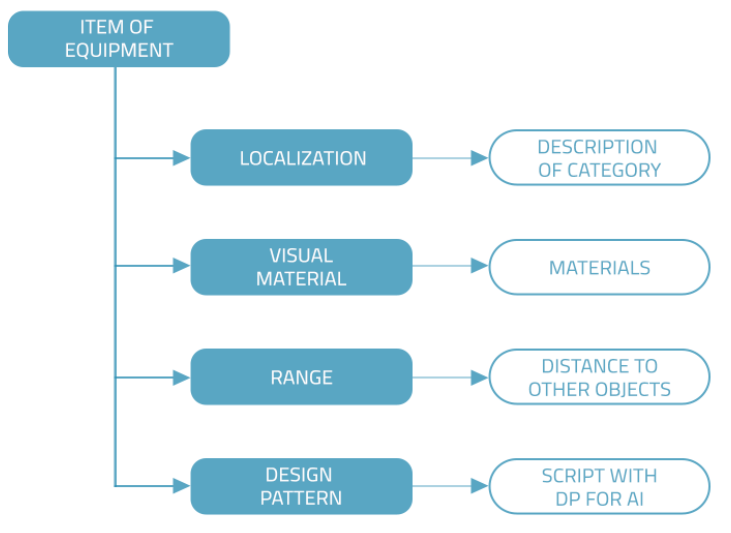
\includegraphics[width=\textwidth]{graf.png}
\caption{Prototyp wykorzystania sztucznej inteligencji w projektowaniu architektonicznym - 
opracowanie własne} \label{fig1}
\end{figure}

Combining individual objects into categories includes in the SVDE, independently parameterized features of objects (Fig. X). Both the list of categories and parameters is expandable. New types of categories can be added as part of the built-in editor, and new types of parameters by adding them in individual implementations.
The basic types of categories include:\\
- bathroom\\
- kitchen\\
- living room\\
- room\\
- living room with kitchen\\
- openings\\

Each of these categories is assigned to IoEs. The basic types of parameters for IoE are:
- location - this parameter contains the specific destination of a given object (a specific category). It is important to be able to assign different locations to one object taking into account the applicable DPs without the need to duplicate a given element depending on the room.
- Material Identification - this parameter is mainly used to define visual appearance of objects. Each of the materials used within the IoE can be declared as a parameter. Materials include elements such as color, transparency, textures, etc. The same material identification parameter can be assigned to multiple IoEs (eg glass texture can be assigned as material to both the window and the door from the shower enclosure).
- Range - this type of parameter is used to define the area of impact of objects within the designed space. It contains information on the need to maintain the appropriate distance from individual objects and the empty space needed for the object to keep. In this case, it is not possible to assign the same parameter to different objects due to the lack of its repeatability in DP.
- Pattern - this type of parameters is used for the creation of aesthetics properties of objects. It contains design patterns that are developed as purely subjective solutions that only make the recipient feel if the space seems to be more or less cozy. 


\section{Podejście SVDE?????}
The SVDE approach has been implemented in IDE and shared repositories. This diagram is presented in Fig. X

\begin{figure}[H]
\centering
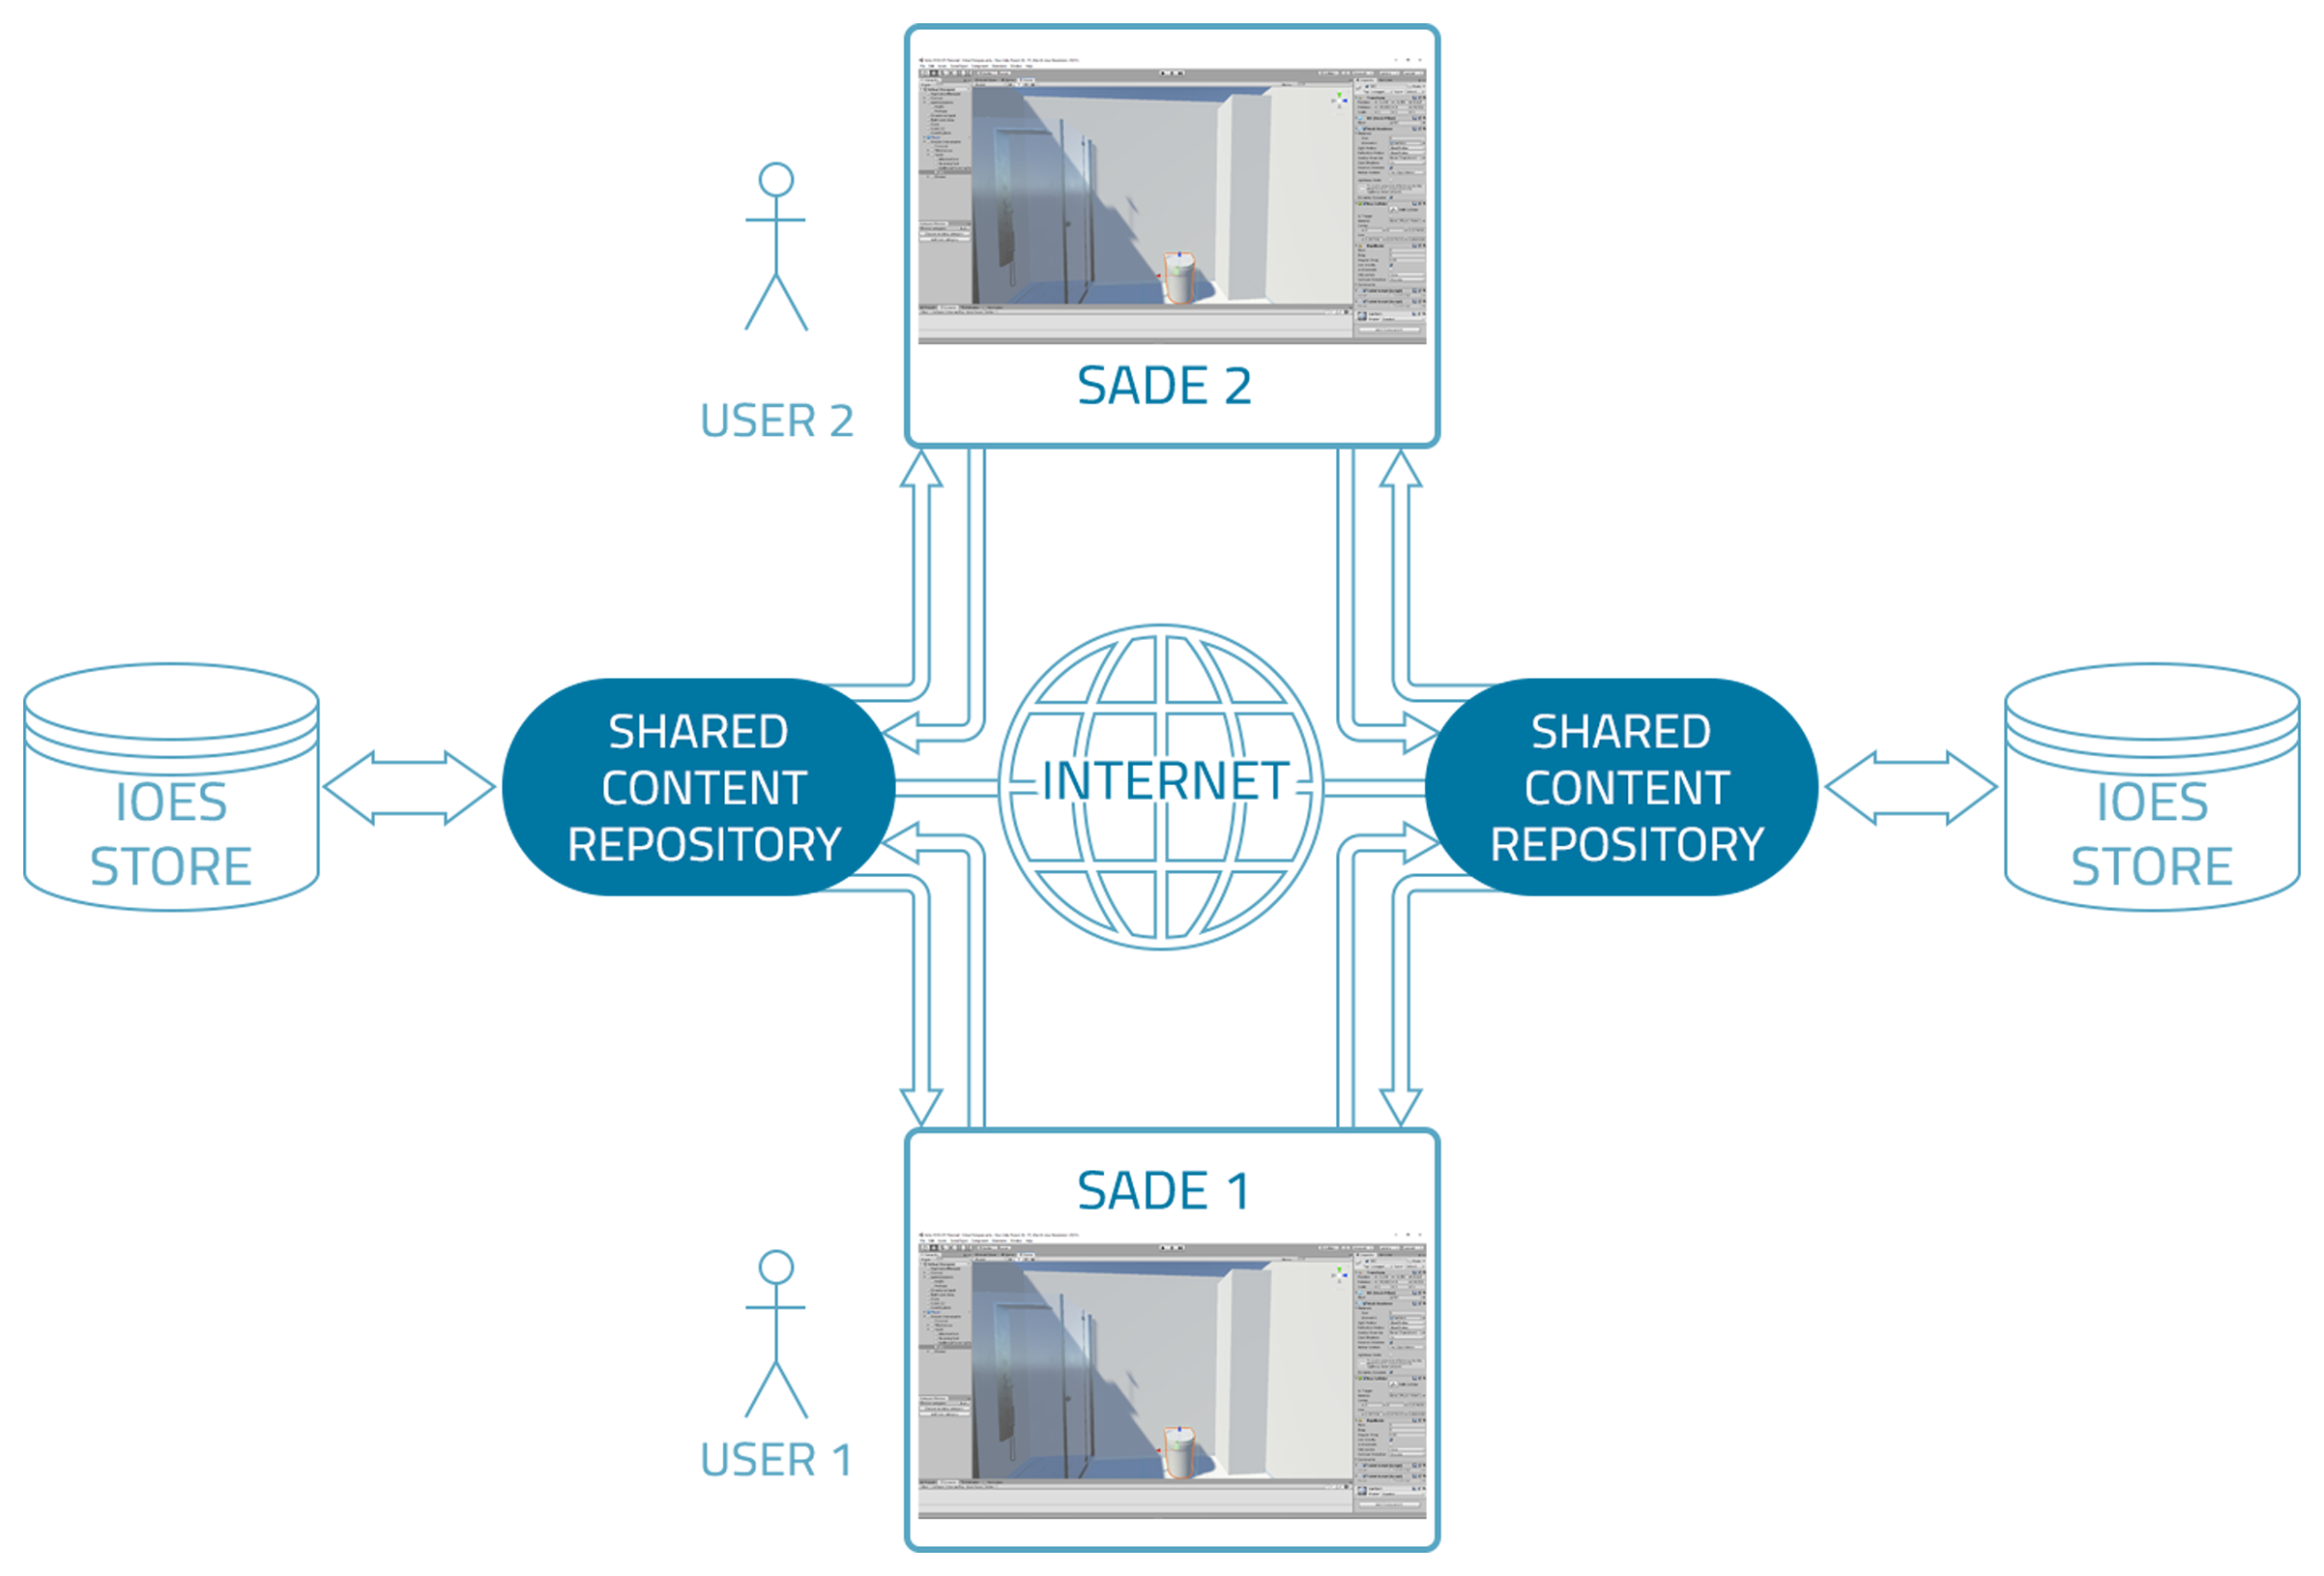
\includegraphics[width=\textwidth]{graf2.png}
\caption{Prototyp wykorzystania sztucznej inteligencji w projektowaniu architektonicznym - 
opracowanie własne} \label{fig2}
\end{figure}
SVDE is implemented in two ways: firstly as an extension to the Unity IDE (figure X), communicating with SCR, which have been implemented as a REST service operating on web servers. The Unity IDE was chosen as the starting point because of its popularity and the multitude of features it has as a cross-platform gaming engine and IDE
[X]. Unity allows you to freely expand with unconventional menus, custom component editors, or editor windows using C\# and JavaScript. The SVDE Unity extension enables the use of virtual rooms (categories) along with their objects, as well as editing or creating resources and sending them in parameterized form to the SCR. This approach was developed based on the SemFlex [X] concept.

The second way to implement the SVDE approach is the application implemented in the framework of the extension that allows the use of fully immersive technology, in which the user has the opportunity to interact directly with the designed space. With the help of previously implemented DPs, all design decisions are monitored by the developed AI, which informs about possible design errors or non-conformities with applicable regulations by means of messages.
Due to the various architectural rules applicable in the world, the relationships between objects such as washing machine - bathtub - toilet are determined using a script written in C\#. Editing individual elements is available from the Unity level, which does not require the user to learn programming knowledge. This allows you to calculate the distance between individual elements relative to the floor of a given room. Below is an example of the method used to calculate these dependencies. 

\begin{lstlisting}[language={[Sharp]C}, caption={C\# exaple}, label={Script}]
public float getDistance()
    {

        return (Vector3.Distance(Element.transform.position, 
        theDuct.transform.position));
    }
\end{lstlisting}

\subsection{Application Example}
Creating a planned space starts with the import of a projection or an empty model and opens the SVDE window allowing the selection of categories. It is available from the menu in Unity. On the left side of the application window there is a hierarchical list of elements within a given scene. At the beginning it contains only basic objects such as: Camera, Point of light, room projection. The bottom left corner of the screen is the open SVDE tool window. The right side of the screen contains a preview of the created 3D scene. The category editor as part of the SVDE tool provides a new one. When the button of the existing category is pressed, a pop-up menu. The list of categories is taken from a DPs shared repository (Fig. X). After selection of the category appears a new window and a scalable box, by means of which the user limits a given space as a specific room. After the user has defined the boundaries of the designed space, the actual design process begins.

\begin{figure}[H]
\centering
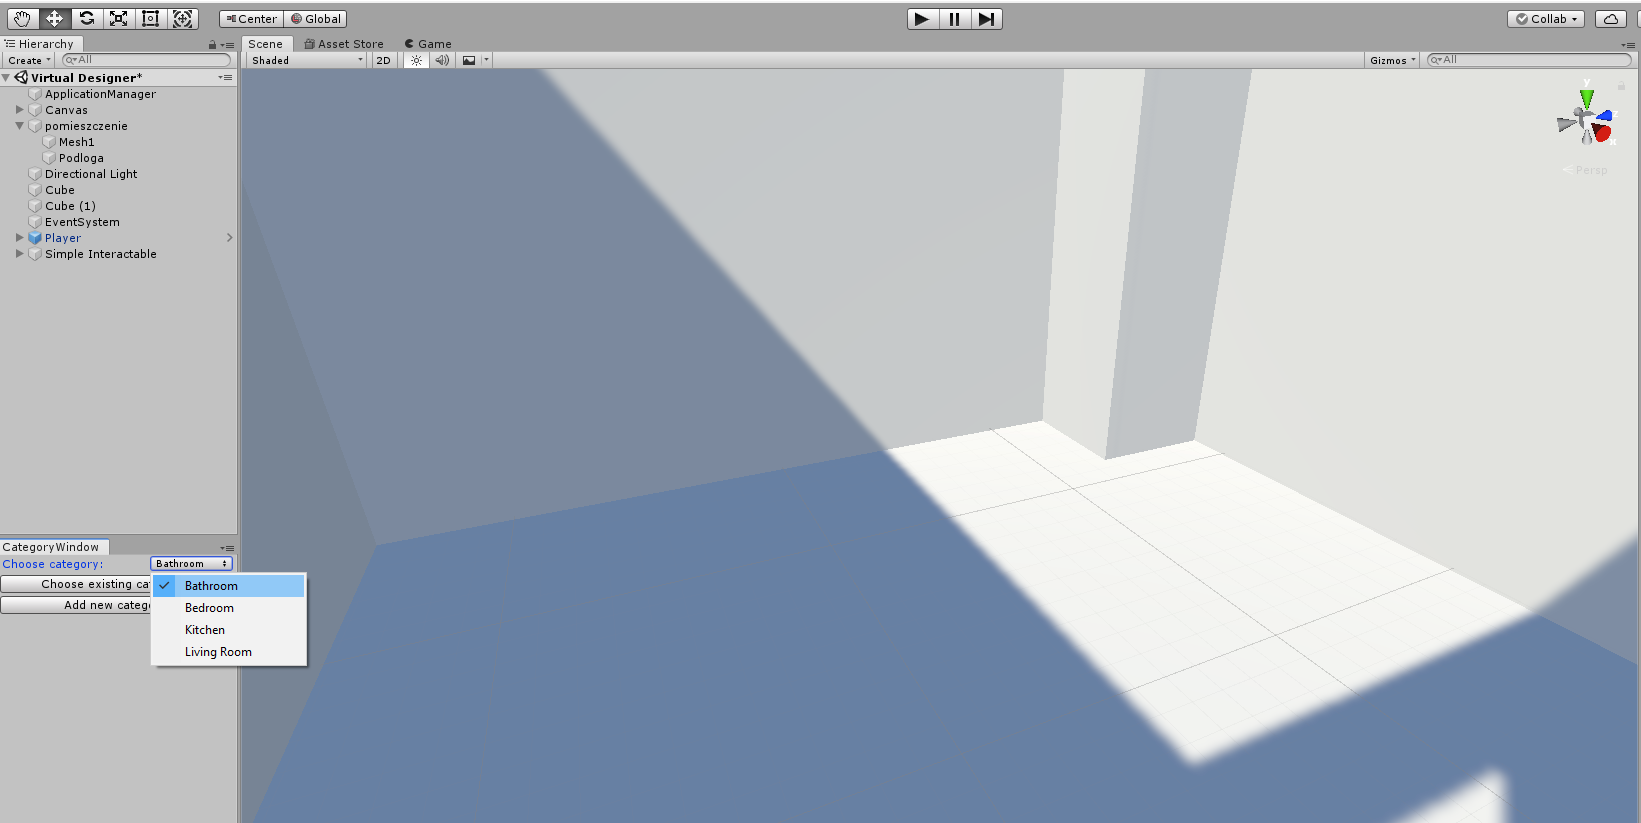
\includegraphics[width=\textwidth, height=5.3cm]{editor1.png}
\caption{Prototyp wykorzystania sztucznej inteligencji w projektowaniu architektonicznym - opracowanie własne} \label{fig3}
\end{figure}

\begin{figure}
     \centering
     \subfloat[][category selection window] {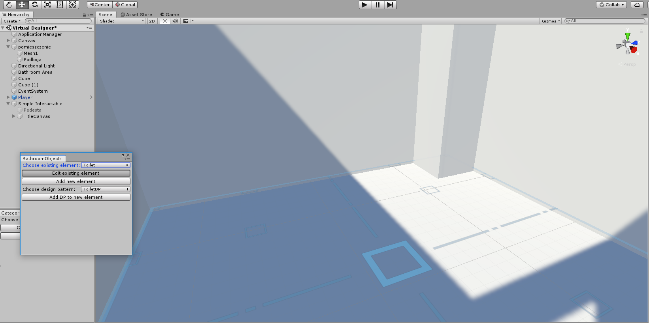
\includegraphics[width=.46\linewidth]{editor2.png}\label{fig4}}%
     \hspace{0.5cm}
     \subfloat[][category  box] {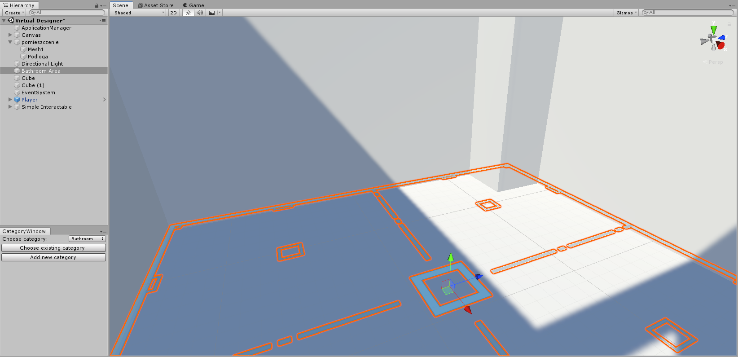
\includegraphics[width=.475\linewidth]{editor3.png}\label{fig5}}
     \caption{Comparison of steady state results (a) x method (b) y method}
     \label{steady_state}
\end{figure}

\begin{figure}[H]
\centering
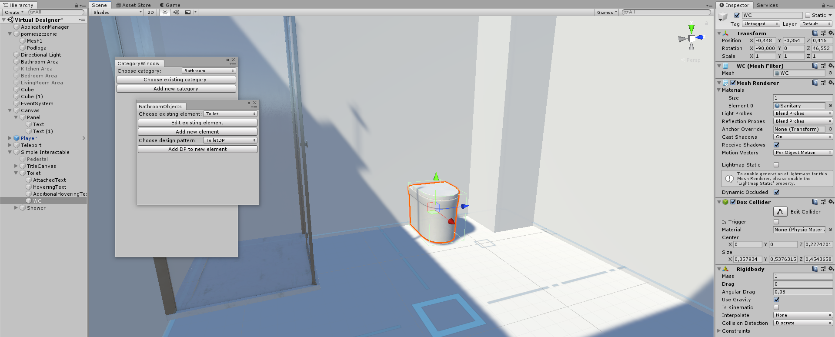
\includegraphics[width=\textwidth, height=4.5cm]{editor4.png}
\caption{Prototyp wykorzystania sztucznej inteligencji w projektowaniu architektonicznym - opracowanie własne} \label{fig6}
\end{figure}

The process consists of several phases. First of all, we need to choose objects that are to be located in the designed space. The objects are downloaded from the server in the form of a package (.unitypackage) along with the DPs file assigned to them. After importing packages with user-oriented objects from the drop-down menu from the application level, it is possible to add individual elements to the room (washing machine, toilet, etc.). With the help of motion controllers, for example HTC Vive, the user can interact with the object he chooses by changing its position, while receiving all the time feedback containing distances from other elements contained in this space, such as shafts.
At the moment when the user makes a decision that is inconsistent with the applicable design rules, he will receive a warning from the system about irregularities with the considered guidelines that generate this error.
In the presented example (Fig. X), the room has been associated with the bathroom category, which as the room inside the flat or house has the most restrictions as to the mutual relations of individual objects and the required distances. The distance parameter which has been assigned to the toilet limits the distance area that can be applied both to the maximum from the board (in this case 1.0 m) and the minimum distance that must be kept (eg 0.3 m from the wall). In the presented example, this object must only have an assigned component specifying its relationship with other elements of equipment.

\begin{figure}[H]
     \centering
     \subfloat[][category selection window] {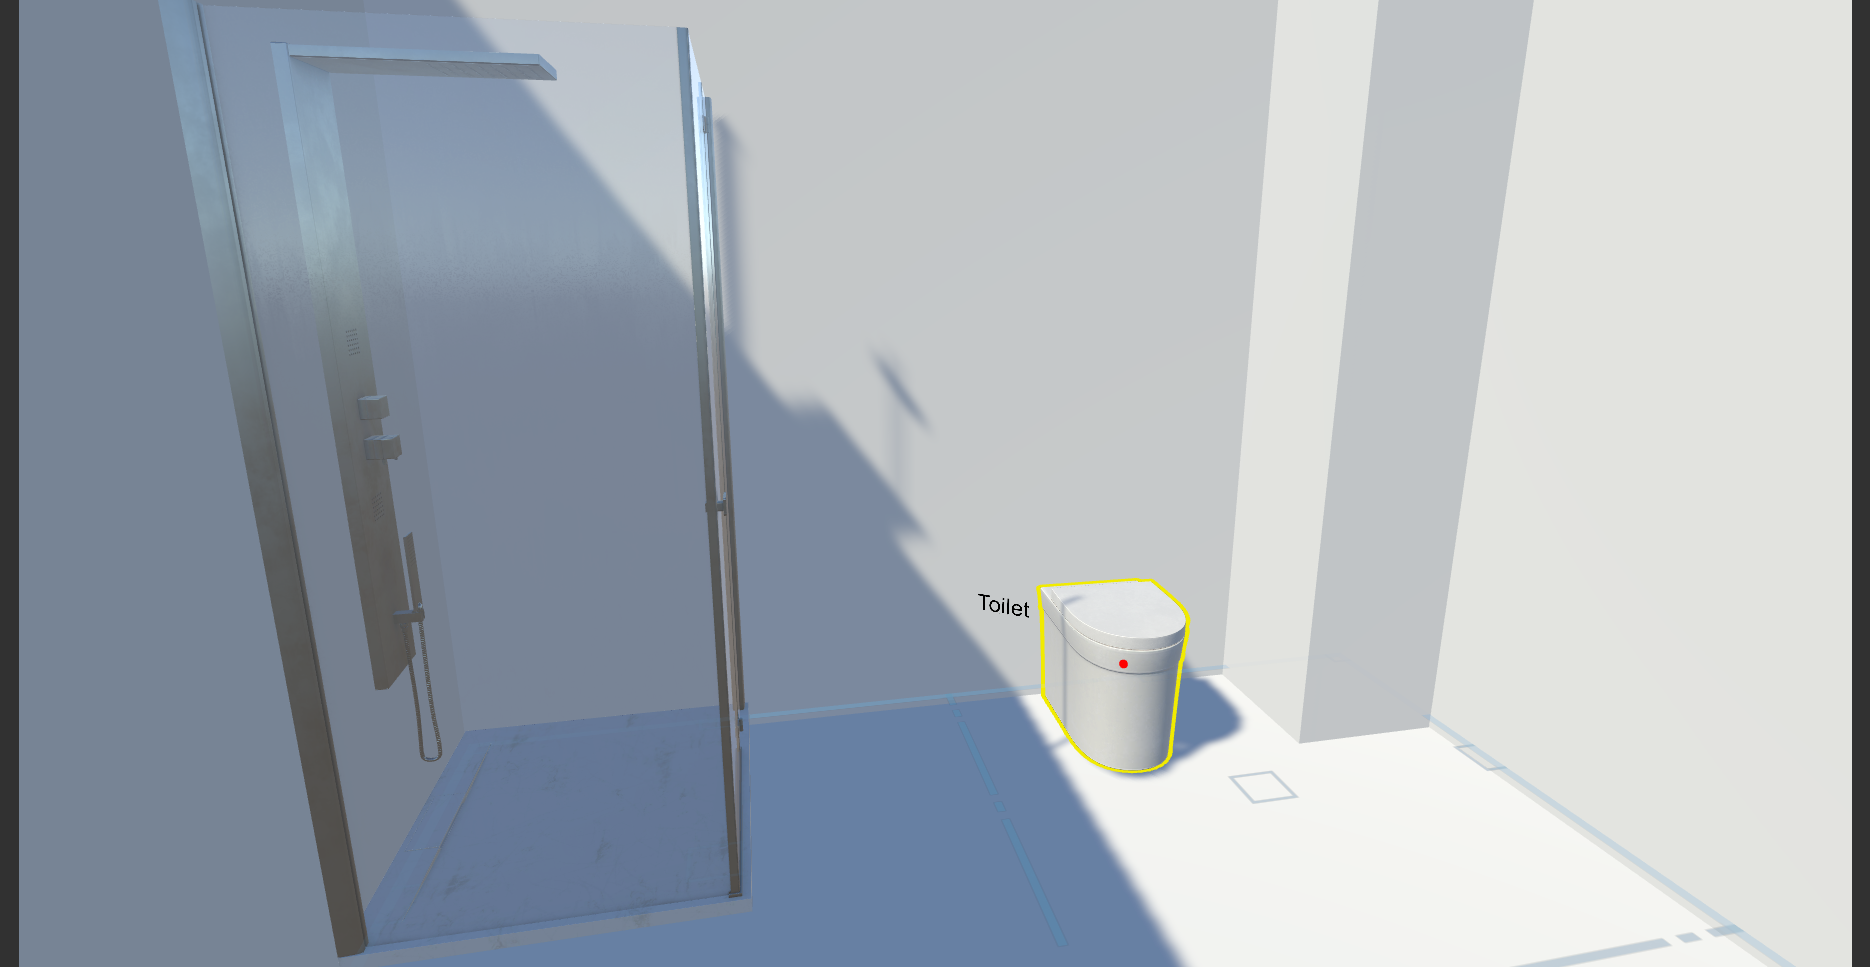
\includegraphics[width=.46\linewidth]{aplikacja1.png}\label{fig4}}%
     \hspace{0.5cm}
     \subfloat[][category  box] {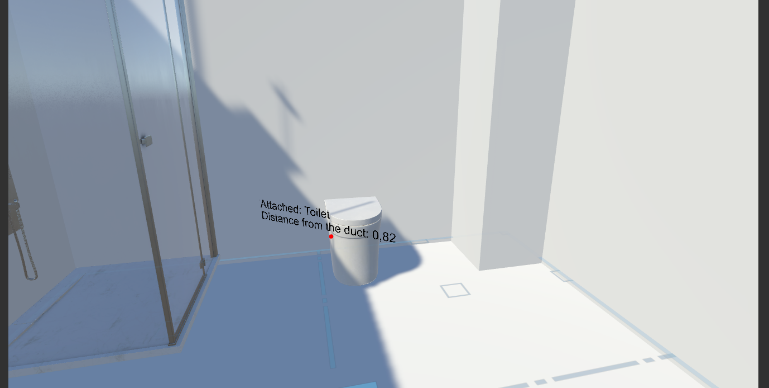
\includegraphics[width=.475\linewidth]{aplikacja2.png}\label{fig5}}
     \caption{Comparison of steady state results (a) x method (b) y method}
     \label{fig7}
\end{figure}

\begin{figure}[H]
\centering
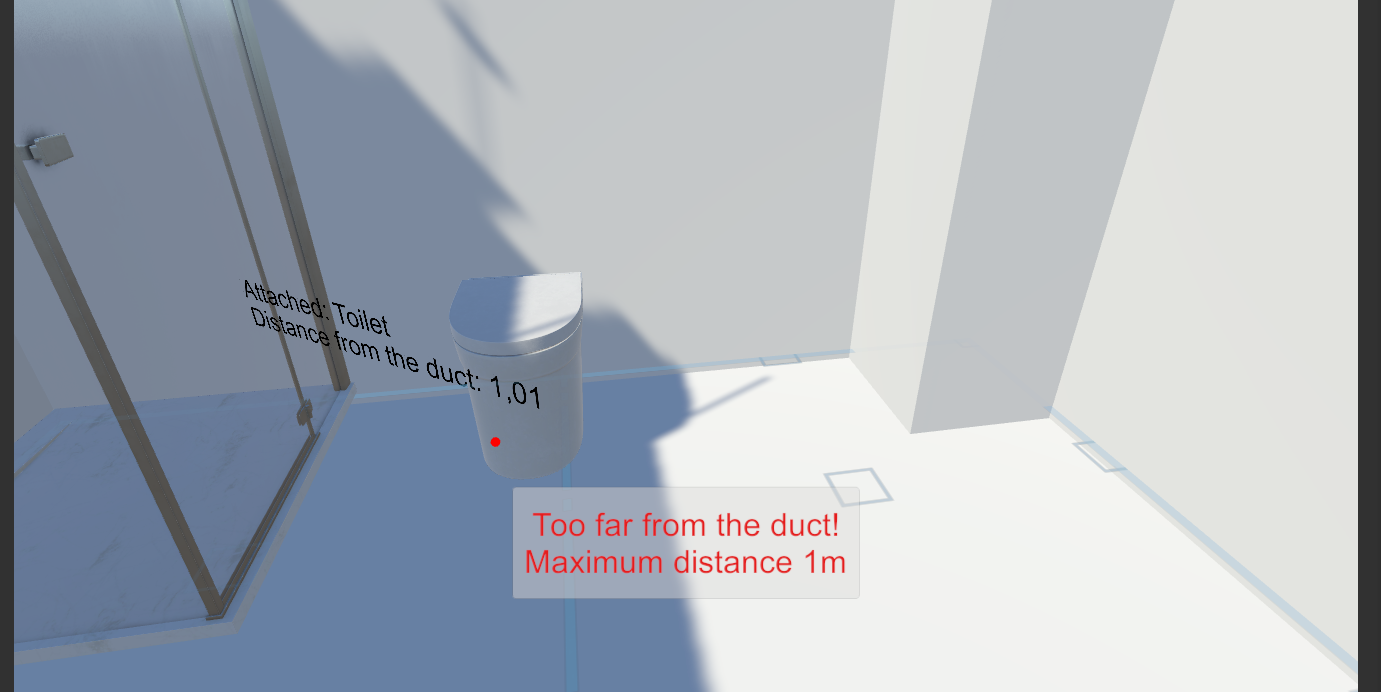
\includegraphics[width=\textwidth]{aplikacja3.png}
\caption{Prototyp wykorzystania sztucznej inteligencji w projektowaniu architektonicznym - 
opracowanie własne} \label{fig8}
\end{figure}


Thanks to this type of approach, the process of space design is simplified by limiting the available elements in a given area, which avoids often obvious design mistakes, and reduces the cost of creating one's own living space due to the fact that no special education is required for people who want to independently design your own living space. Thanks to the use of shared repositories, it is possible to use a wide range of products available on the market.

\subsection{Future works}
At a later stage of developing the application, an important point to enter is creating a plug-in installed in 3D content creation programs that will allow you to standardize the extension for imported objects. Thanks to this, it will be possible to avoid deficiencies in export-based models. The second direction of development is to expand the competence of AI by being able to independently propose layouts of elements within a given room, using the existing solutions. This will allow even more ergonomic development of the living space. And the last direction at this stage is to enable the repository to download ready-made solutions for rooms that will only require minor editing.

\section{Conclusion}
This article presents a new approach to the design of architectural spaces. The approach, called SVDE, is based on the concept of parameterization of content - semantically described objects, which are the basic unit ready to be shared. The method is flexible, because it allows both the transition from parameterized to categorized content, and vice versa, i.e. providing the ability to use existing content libraries to be used or edited to create final virtual scenes. Thanks to such a mechanism, it is possible to create social content in 3D. The content creation process takes place in a dispersed architecture. Thanks to the generally available elements, the design process is shortened mainly to the selection of the user's interesting elements to be placed in the designed space. The design process is simplified by the semantics of use. Taxonomy is used to describe the classes of objects. These classes are used to define ranges of values of IoE parameters and their DPs, thus reducing the complexity of artificial intelligence used to detect possible irregularities. Currently, the semantic IDE - implemented as an extension of the editor to the Unity IDE - ensures creation of IoEs semantic instances in the wizard, importing content from SCR, and creating parameterized ToR categories from existing content elements. Parameterization of the created IoE is done manually, through the window editor of the generated code containing design patterns. In future work, it is planned to extend the application to a fully functional AI, capable of making independent decisions. This will further simplify the design process. The presented method of building semantic parameterized content elements and their creation has been tested with a limited number of relatively simple design scenarios. In future works, a larger design sample is planned that will require more related elements

%For citations of references, we prefer the use of square brackets
%and consecutive numbers. Citations using labels or the author/year
%convention are also acceptable. The following bibliography provides
%a sample reference list with entries for journal
%articles~\cite{ref_article1}, an LNCS chapter~\cite{ref_lncs1}, a
%book~\cite{ref_book1}, proceedings without editors~\cite{ref_proc1},
%and a homepage~\cite{ref_url1}. Multiple citations are grouped
%\cite{ref_article1,ref_lncs1,ref_book1},
%\cite{ref_article1,ref_book1,ref_proc1,ref_url1}.
%
% ---- Bibliography ----
%
% BibTeX users should specify bibliography style 'splncs04'.
% References will then be sorted and formatted in the correct style.
%
% \bibliographystyle{splncs04}
% \bibliography{mybibliography}
%
\begin{thebibliography}{8}
\bibitem{ref_article1}
Author, F.: Article title. Journal \textbf{2}(5), 99--110 (2016)

\bibitem{ref_lncs1}
Author, F., Author, S.: Title of a proceedings paper. In: Editor,
F., Editor, S. (eds.) CONFERENCE 2016, LNCS, vol. 9999, pp. 1--13.
Springer, Heidelberg (2016). \doi{10.10007/1234567890}

\bibitem{ref_book1}
Author, F., Author, S., Author, T.: Book title. 2nd edn. Publisher,
Location (1999)

\bibitem{ref_proc1}
Author, A.-B.: Contribution title. In: 9th International Proceedings
on Proceedings, pp. 1--2. Publisher, Location (2010)

\bibitem{ref_url1}
LNCS Homepage, \url{http://www.springer.com/lncs}. Last accessed 4
Oct 2017

\bibitem{ref_article1}
Author, F.: Article title. Journal \textbf{2}(5), 99--110 (2016)

\bibitem{ref_lncs1}
Author, F., Author, S.: Title of a proceedings paper. In: Editor,
F., Editor, S. (eds.) CONFERENCE 2016, LNCS, vol. 9999, pp. 1--13.
Springer, Heidelberg (2016). \doi{10.10007/1234567890}

\bibitem{ref_book1}
Author, F., Author, S., Author, T.: Book title. 2nd edn. Publisher,
Location (1999)

\bibitem{ref_proc1}
Author, A.-B.: Contribution title. In: 9th International Proceedings
on Proceedings, pp. 1--2. Publisher, Location (2010)

\bibitem{ref_url1}
LNCS Homepage, \url{http://www.springer.com/lncs}. Last accessed 4
Oct 2017

\bibitem{ref_article1}
Author, F.: Article title. Journal \textbf{2}(5), 99--110 (2016)

\bibitem{ref_lncs1}
Author, F., Author, S.: Title of a proceedings paper. In: Editor,
F., Editor, S. (eds.) CONFERENCE 2016, LNCS, vol. 9999, pp. 1--13.
Springer, Heidelberg (2016). \doi{10.10007/1234567890}

\bibitem{ref_book1}
Author, F., Author, S., Author, T.: Book title. 2nd edn. Publisher,
Location (1999)

\bibitem{ref_proc1}
Author, A.-B.: Contribution title. In: 9th International Proceedings
on Proceedings, pp. 1--2. Publisher, Location (2010)

\bibitem{ref_url1}
LNCS Homepage, \url{http://www.springer.com/lncs}. Last accessed 4
Oct 2017

\bibitem{ref_article1}
Author, F.: Article title. Journal \textbf{2}(5), 99--110 (2016)

\bibitem{ref_lncs1}
Author, F., Author, S.: Title of a proceedings paper. In: Editor,
F., Editor, S. (eds.) CONFERENCE 2016, LNCS, vol. 9999, pp. 1--13.
Springer, Heidelberg (2016). \doi{10.10007/1234567890}

\bibitem{ref_book1}
Author, F., Author, S., Author, T.: Book title. 2nd edn. Publisher,
Location (1999)

\bibitem{ref_proc1}
Author, A.-B.: Contribution title. In: 9th International Proceedings
on Proceedings, pp. 1--2. Publisher, Location (2010)

\bibitem{ref_url1}
LNCS Homepage, \url{http://www.springer.com/lncs}. Last accessed 4
Oct 2017

\bibitem{ref_article1}
Author, F.: Article title. Journal \textbf{2}(5), 99--110 (2016)

\bibitem{ref_lncs1}
Author, F., Author, S.: Title of a proceedings paper. In: Editor,
F., Editor, S. (eds.) CONFERENCE 2016, LNCS, vol. 9999, pp. 1--13.
Springer, Heidelberg (2016). \doi{10.10007/1234567890}

\bibitem{ref_book1}
Author, F., Author, S., Author, T.: Book title. 2nd edn. Publisher,
Location (1999)

\bibitem{ref_proc1}
Author, A.-B.: Contribution title. In: 9th International Proceedings
on Proceedings, pp. 1--2. Publisher, Location (2010)

\bibitem{ref_url1}
LNCS Homepage, \url{http://www.springer.com/lncs}. Last accessed 4
Oct 2017
\end{thebibliography}
\end{document}
